% ============================================================
%  N.3.3  Fixed-Config Scaling — Energy Ratio vs Register Size
% ============================================================
\subsection{Fixed-Config Scaling: Energy Ratio vs.\ Register Size
  (Eyeriss)}
\label{sec:fusion-fixed-scaling}

\subsubsection{Motivation}

Sections~\ref{sec:fusion-full-sized} and~\ref{sec:fusion-partial-sized}
compared fusion modes at a single architecture point per workload.
A natural question is how the energy penalty of fusion \emph{scales}
as the per-PE register grows.
CS1 (Section~\ref{sec:eyeriss-cs1}) showed that the minimum feasible
WReg doubles with every halving of the PE count, because the
weight footprint that each PE must carry increases in proportion.
The energy cost of each register access also scales with register
size, so one expects the fusion-to-single energy ratio to grow
with WReg.
This section quantifies that growth by sweeping three PE
configurations on the Eyeriss architecture, each requiring
progressively larger registers.

Two weight-dominant workloads, ResNet18 and VGG16, are examined
because they span a range of WReg values wide enough to reveal
the scaling trend.
For each workload, three PE counts are tested
(16\,384, 8\,192, 4\,096), each paired with the minimum WReg
determined by CS1.
The activation-dominant workloads (FSRCNN, MC-CNN) are excluded
from the sweep because they share a single WReg\,=\,384
regardless of PE count, so there is no register-size axis to
sweep.

\subsubsection{Results}

\paragraph{ResNet18 (Figure~\ref{fig:fusion-fixed-resnet18}).}
Table~\ref{tab:fusion-fixed-resnet18} reports the three
configurations.
At the largest array ($512 \times 32$, 16\,384~PEs, WReg\,=\,902)
the full-to-single energy ratio is $8.0\times$.
Halving the PE count to 8\,192 and doubling WReg to 1\,800
raises the ratio to $11.7\times$, a $1.5\times$ increase.
At 4\,096~PEs with WReg\,=\,3\,600, the ratio reaches
$19.6\times$.

\begin{table}[htbp]
  \centering
  \caption{Eyeriss fixed-config scaling for ResNet18 (Scenario~A).
    WReg is the minimum feasible value from CS1.
    Energy ratio\,=\,Full\,/\,Single.}
  \label{tab:fusion-fixed-resnet18}
  \begin{tabular}{lrrrrrr}
    \toprule
    Config & PEs & WReg
      & Full ($\mu$J) & Single ($\mu$J)
      & Ratio \\
    \midrule
    $512 \times 32$  & 16\,384 &    902
      & $2.37 \times 10^{4}$ & $2.98 \times 10^{3}$
      & $8.0\times$ \\
    $256 \times 32$  &  8\,192 &  1\,800
      & $3.25 \times 10^{4}$ & $2.78 \times 10^{3}$
      & $11.7\times$ \\
    $256 \times 16$  &  4\,096 &  3\,600
      & $5.20 \times 10^{4}$ & $2.65 \times 10^{3}$
      & $19.6\times$ \\
    \bottomrule
  \end{tabular}
\end{table}

The growth arises because two effects stack in the ratio.
First, the fused energy increases with WReg because every
register access touches a larger SRAM structure, and the
aggregate register capacity across all PEs is roughly constant
($902 \times 16{,}384 \approx 14.8$\,M~words at the top,
$3{,}600 \times 4{,}096 \approx 14.7$\,M at the bottom), so the
per-access cost rises while the total capacity stays flat.
Second, the single-layer energy \emph{decreases} slightly with
fewer PEs because single-layer mode does not require the
oversized WReg.
However, the single-layer shrinkage is modest (only
$5$--$13\%$ per step) because the DRAM component of single-layer
energy is substantial and PE-count-independent, leaving the
register-driven reduction as a minor effect.
The ratio growth is therefore driven primarily by the
fused-energy increase ($1.4$--$1.7\times$ per step).

\begin{figure}[htbp]
  \centering
  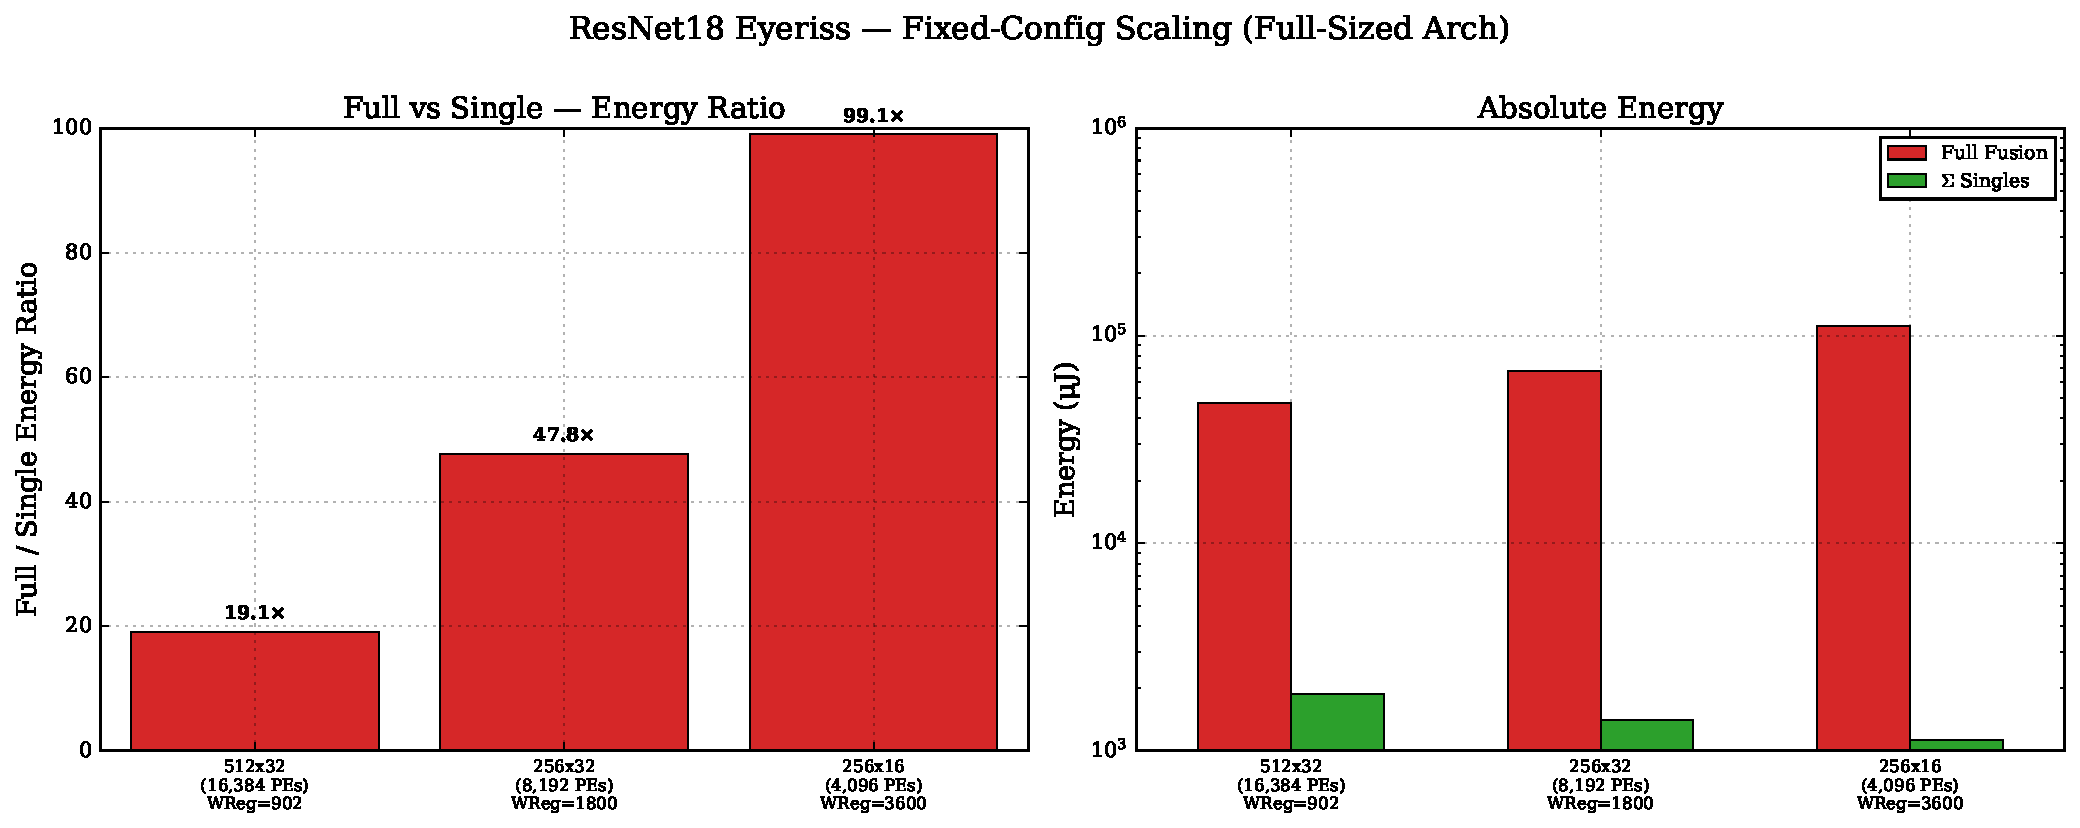
\includegraphics[width=0.95\textwidth]{plots/fusion_fixed_resnet18_scaling.pdf}
  \caption{Eyeriss fixed-config scaling for ResNet18.
    Left: full-to-single energy ratio.
    Right: absolute energy on a log scale.}
  \label{fig:fusion-fixed-resnet18}
\end{figure}

\paragraph{VGG16 (Figure~\ref{fig:fusion-fixed-vgg16}).}
VGG16 exhibits the same pattern, amplified by its larger register
requirements.
At WReg\,=\,1\,200 (16\,384~PEs) the ratio is $17.0\times$;
at WReg\,=\,2\,400 (8\,192~PEs) it rises to $28.9\times$; and at
WReg\,=\,4\,800 (4\,096~PEs) it reaches $54.1\times$.
Each doubling step grows the ratio by $1.7$--$1.9\times$,
consistent with the ResNet18 trend.

\begin{table}[htbp]
  \centering
  \caption{Eyeriss fixed-config scaling for VGG16 (Scenario~A).}
  \label{tab:fusion-fixed-vgg16}
  \begin{tabular}{lrrrrrr}
    \toprule
    Config & PEs & WReg
      & Full ($\mu$J) & Single ($\mu$J)
      & Ratio \\
    \midrule
    $512 \times 32$  & 16\,384 &  1\,200
      & $1.63 \times 10^{5}$ & $9.59 \times 10^{3}$
      & $17.0\times$ \\
    $256 \times 32$  &  8\,192 &  2\,400
      & $2.45 \times 10^{5}$ & $8.49 \times 10^{3}$
      & $28.9\times$ \\
    $256 \times 16$  &  4\,096 &  4\,800
      & $4.19 \times 10^{5}$ & $7.74 \times 10^{3}$
      & $54.1\times$ \\
    \bottomrule
  \end{tabular}
\end{table}

VGG16 also reveals a difference between full and partial fusion.
The full-to-partial energy ratio is $2.55\times$ at
WReg\,=\,1\,200 and decreases to $1.41\times$ at
WReg\,=\,4\,800, indicating that as registers grow, partial
fusion captures most of the fused-mode overhead and the gap
between the two modes narrows.
For ResNet18 the full-to-partial ratio ranges from $1.44\times$
at the smallest WReg down to $1.02\times$ at the largest,
showing near-equivalent energy for full and partial fusion at
large registers.

\begin{figure}[htbp]
  \centering
  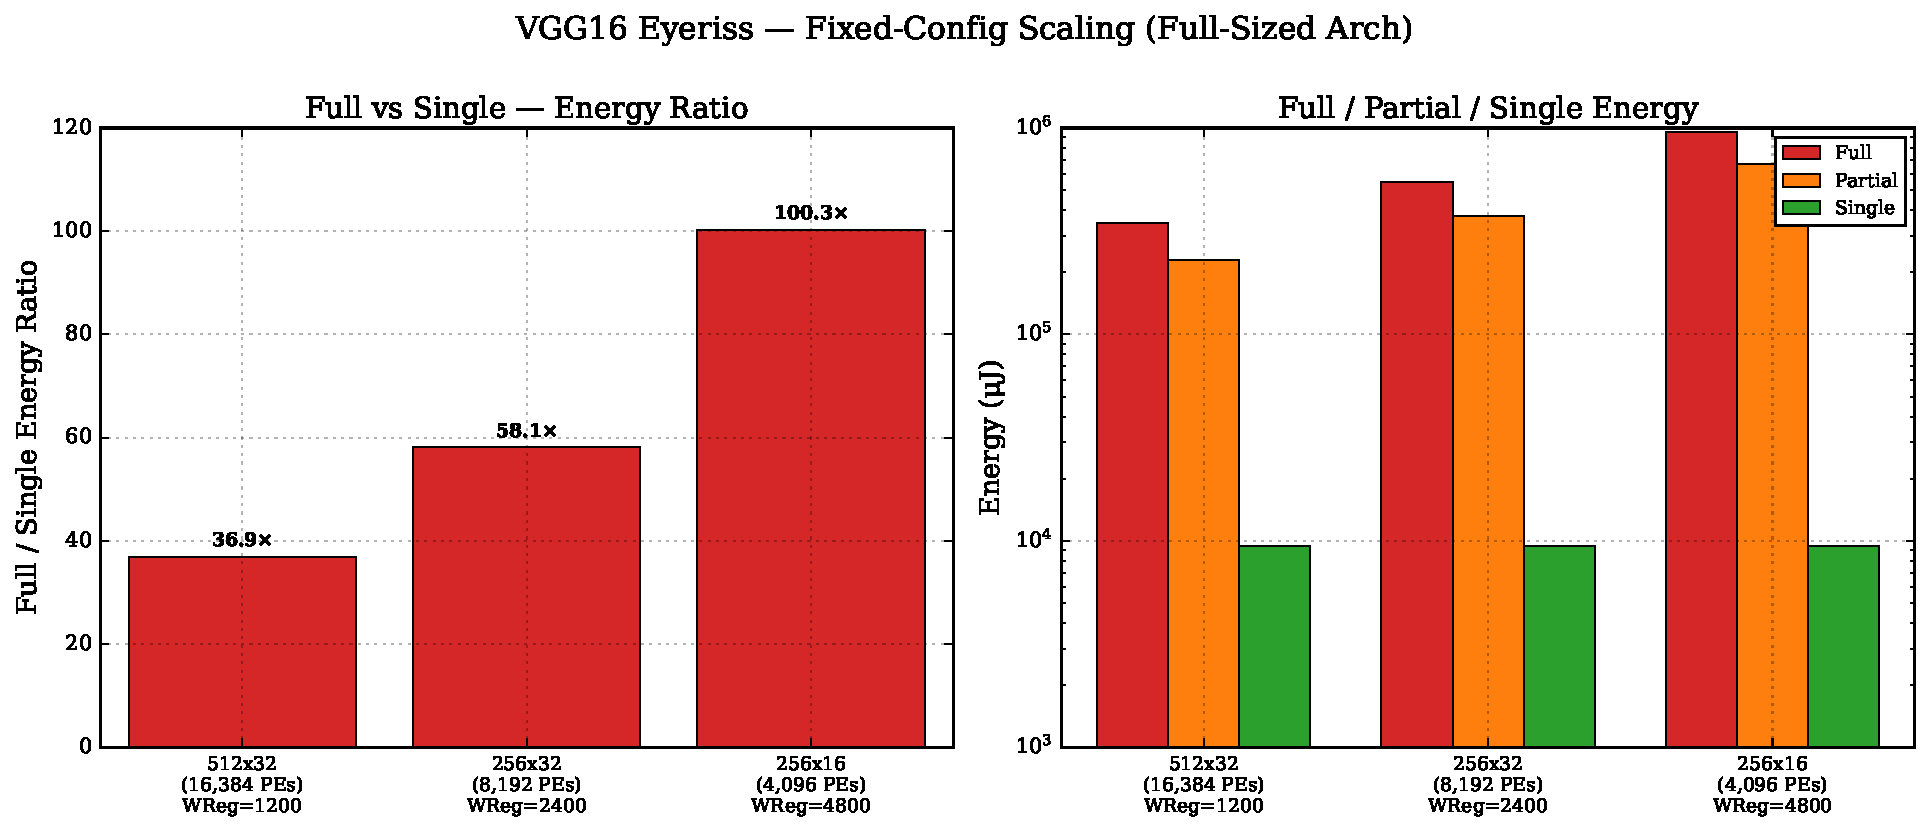
\includegraphics[width=0.95\textwidth]{plots/fusion_fixed_vgg16_scaling.pdf}
  \caption{Eyeriss fixed-config scaling for VGG16.
    Left: full-to-single energy ratio.
    Right: absolute energy (full, partial, single) on a log scale.}
  \label{fig:fusion-fixed-vgg16}
\end{figure}

\paragraph{Activation-dominant workloads.}
FSRCNN and MC-CNN do not participate in this sweep because their
WReg remains at 384~words regardless of the PE configuration.
At that single operating point, the full-to-single energy ratios
are $1.0\times$ (FSRCNN) and $2.2\times$ (MC-CNN), which
sit well below the weight-dominant ratios.
For FSRCNN, fusion incurs essentially no energy overhead: almost
all energy is spent in DRAM transfers that are common to both
modes.
The constant WReg reflects the fact that, for shallow networks
with small filter counts, the per-PE weight footprint is already
negligible at the minimum PE count.

\paragraph{Scaling rule.}
Across both workloads, each $2\times$ increase in WReg raises
the fusion-to-single energy ratio by a factor of roughly
$1.5$--$1.9\times$.
The fused energy grows by $1.4$--$1.7\times$ per WReg step
because each register access touches a larger SRAM structure.
The single-layer energy shrinks only modestly, by
$1.05$--$1.13\times$, because the DRAM component of single-layer
energy is substantial and PE-count-independent, so the
register-driven shrinkage is a minor effect.
The product of these two factors yields the observed
${\sim}1.5$--$1.9\times$ ratio growth per step.

\paragraph{Considerations}
The energy penalty of fusion on the Eyeriss architecture is not a
fixed constant; it \emph{scales super-linearly} with register size.
A designer who chooses a smaller PE array to save area will face a
correspondingly larger WReg and, consequently, a worse
fusion-to-single energy ratio.
At the extreme tested point (VGG16, WReg\,=\,4\,800), fusion
consumes $54\times$ the energy of single-layer execution.
This scaling behavior reinforces the conclusion from
Sections~\ref{sec:fusion-full-sized}
and~\ref{sec:fusion-partial-sized}: fusion's energy cost is
the dominant factor in the EDP trade-off, and it grows worse
as the architecture is scaled down.